\chapter{Platform-Level Interrupt Controller (PLIC)}
\label{plic}

This chapter describes the general architecture for the RISC-V
platform-level interrupt controller (PLIC), which prioritizes and
distributes global interrupts in a RISC-V system.

\section{PLIC Overview}

Figure~\ref{fig:plic} provides a quick overview of PLIC operation.
The PLIC connects global {\em interrupt sources}, which are usually
I/O devices, to {\em interrupt targets}, which are usually {\em hart
  contexts}.  The PLIC contains multiple {\em interrupt gateways}, one
per interrupt source, together with a {\em PLIC core} that performs
interrupt prioritization and routing.  Global interrupts are sent from
their source to an {\em interrupt gateway} that processes the
interrupt signal from each source and sends a single {\em interrupt
  request} to the PLIC core, which latches these in the core interrupt
pending bits (IP).  Each interrupt source is assigned a separate
priority.  The PLIC core contains a matrix of interrupt enable (IE)
bits to select the interrupts that are enabled for each target.  The
PLIC core forwards an {\em interrupt notification} to one or more
targets if the targets have any pending interrupts enabled, and the
priority of the pending interrupts exceeds a per-target threshold.
When the target takes the external interrupt, it sends an {\em
  interrupt claim} request to retrieve the identifier of the
highest-priority global interrupt source pending for that target from
the PLIC core, which then clears the corresponding interrupt source
pending bit.  After the target has serviced the interrupt, it sends
the associated interrupt gateway an {\em interrupt completion} message
and the interrupt gateway can now forward another interrupt request
for the same source to the PLIC.  The rest of this chapter describes
each of these components in detail, though many details are
necessarily platform specific.

\begin{figure}[tb]
\centering
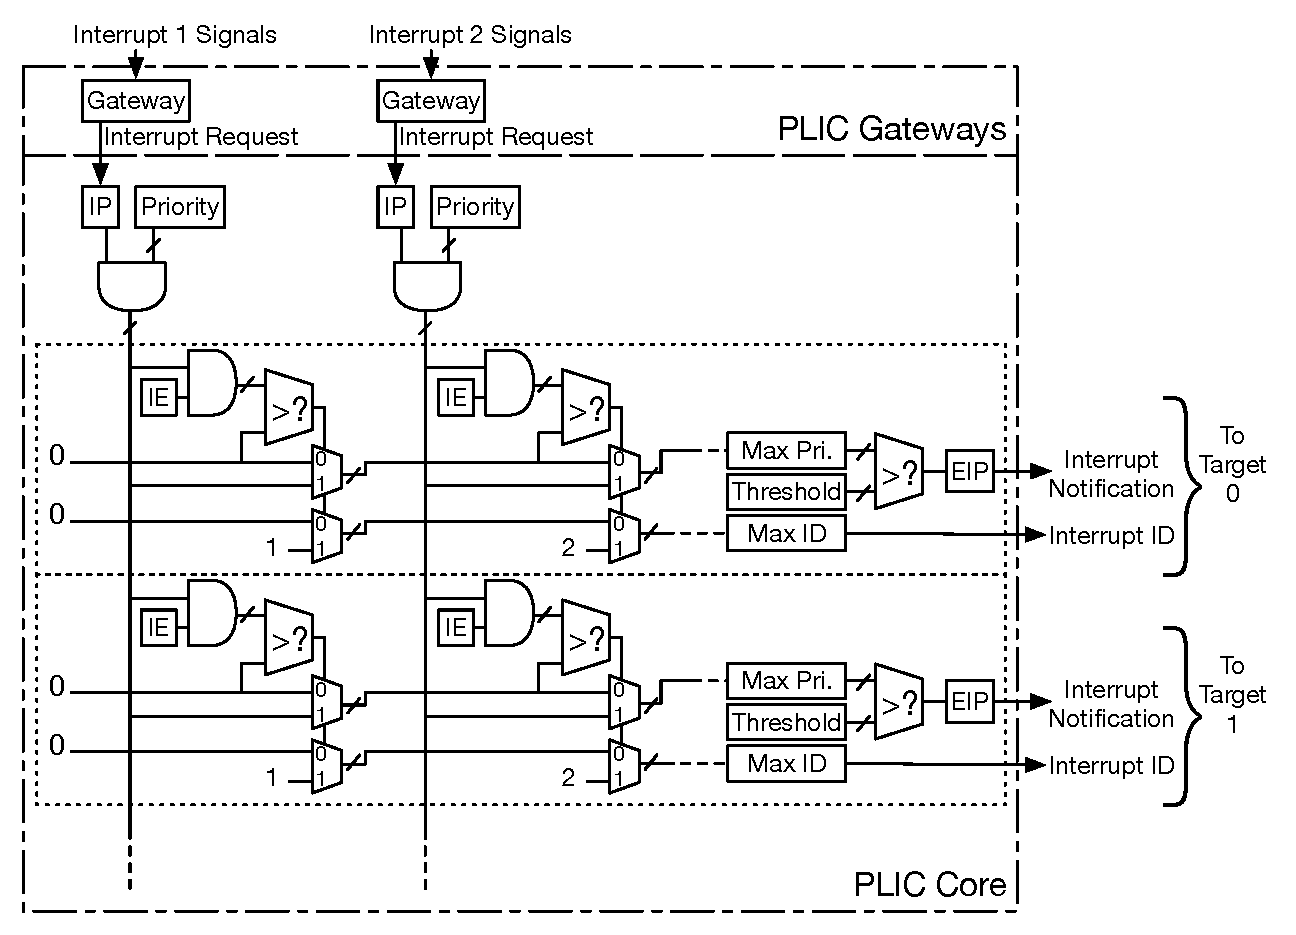
\includegraphics[width=\textwidth]{figs/PLIC-block-diagram.pdf}
\caption{Platform-Level Interrupt Controller (PLIC) conceptual block
  diagram.  The figure shows the first two of potentially many
  interrupt sources, and the first two of potentially many interrupt
  targets.  The figure is just intended to show the logic of the
  PLIC's operation, not to represent a realistic implementation
  strategy.}
\label{fig:plic}
\end{figure}

\section{Interrupt Sources}

RISC-V harts can have both local and global interrupt sources.  Only
global interrupt sources are handled by the PLIC.

\subsection{Local Interrupt Sources}

Each hart has a number of {\em local interrupt sources} that do not
pass through the PLIC, including the standard software interrupts and
timer interrupts for each privilege level.  Local interrupts can be
serviced quickly since there will be minimal latency between the
source and the servicing hart, no arbitration is required to determine
which hart will service the request, and the servicing hart can
quickly determine the interrupt source using the {\tt mcause}
register.

All local interrupts follow a level-based model, where an interrupt is
pending if the corresponding bit in {\tt mip} is set.  The interrupt
handler must clear the hardware condition that is causing the {\tt
  mip} bit to be set to avoid retaking the interrupt after re-enabling
interrupts on exit from the interrupt handler.

Additional non-standard local interrupt sources can be made visible to
machine-mode by adding them to the high bits of the {\tt mip}/{\tt
  mie} registers, with corresponding additional cause values returned
in the {\tt mcause} register.  These additional non-standard local
interrupts may also be made visible to lower privilege levels, using
the corresponding bits in the {\tt mideleg} register.  The priority of
non-standard local interrupt sources relative to external, timer, and
software interrupts is platform-specific.

\subsection{Global Interrupt Sources}

{\em Global interrupt sources} are those that are prioritized and
distributed by the PLIC.  Depending on the platform-specific PLIC
implementation, any global interrupt source could be routed to any
hart context.

Global interrupt sources can take many forms, including
level-triggered, edge-triggered, and message-signalled.  Some sources
might queue up a number of interrupt requests.  All global interrupt
sources are converted to a common interrupt request format for the
PLIC.

\section{Interrupt Targets and Hart Contexts}

Interrupt targets are usually hart contexts, where a hart context is a
given privilege mode on a given hart (though there are other possible
interrupt targets, such as DMA engines).  Not all hart contexts need
be interrupt targets, in particular, if a processor core does not
support delegating external interrupts to lower-privilege modes, then
the lower-privilege hart contexts will not be interrupt targets.
Interrupt notifications generated by the PLIC appear in the {\tt
  meip}/{\tt seip}/{\tt ueip} bits of the {\tt mip}/{\tt sip}/{\tt
  uip} registers for M/S/U modes respectively.  The notifications
only appear in lower-privilege {\em x}{\tt ip} registers if external
interrupts have been delegated to the lower-privilege modes.

Each processor core must define a policy on how simultaneous active
interrupts are taken by multiple hart contexts on the core. For the
simple case of a single stack of hart contexts, one for each supported
privileged mode, interrupts for higher-privilege contexts can preempt
execution of interrupt handlers for lower-privilege contexts.  A
multithreaded processor core could run multiple independent interrupt
handlers on different hart contexts at the same time.  A processor
core could also provide hart contexts that are only used for interrupt
handling to reduce interrupt service latency, and these might preempt
interrupt handlers for other harts on the same core.

The PLIC treats each interrupt target independently and does not take
into account any interrupt prioritization scheme used by a component
that contains multiple interrupt targets.  As a result, the PLIC
provides no concept of interrupt preemption or nesting so this must be
handled by the cores hosting multiple interrupt target contexts.

\section{Interrupt Gateways}

The interrupt gateways are responsible for converting global interrupt
signals into a common interrupt request format, and for controlling
the flow of interrupt requests to the PLIC core.  At most one
interrupt request per interrupt source can be pending in the PLIC core
at any time, indicated by setting the source's IP bit.  The gateway
only forwards a new interrupt request to the PLIC core after receiving
notification that the interrupt handler servicing the previous
interrupt request from the same source has completed.

If the global interrupt source uses level-sensitive interrupts, the
gateway will convert the first assertion of the interrupt level into
an interrupt request, but thereafter the gateway will not forward an
additional interrupt request until it receives an interrupt completion
message.  On receiving an interrupt completion message, if the
interrupt is level-triggered and the interrupt is still asserted, a
new interrupt request will be forwarded to the PLIC core.  The gateway
does not have the facility to retract an interrupt request once
forwarded to the PLIC core.  If a level-sensitive interrupt source
deasserts the interrupt after the PLIC core accepts the request and
before the interrupt is serviced, the interrupt request remains
present in the IP bit of the PLIC core and will be serviced by a
handler, which will then have to determine that the interrupt device
no longer requires service.

If the global interrupt source was edge-triggered, the gateway will
convert the first matching signal edge into an interrupt request.
Depending on the design of the device and the interrupt handler,
inbetween sending an interrupt request and receiving notice of its
handler's completion, the gateway might either ignore additional
matching edges or increment a counter of pending interrupts.  In
either case, the next interrupt request will not be forwarded to the
PLIC core until the previous completion message has been received.  If
the gateway has a pending interrupt counter, the counter will be
decremented when the interrupt request is accepted by the PLIC core.

Unlike dedicated-wire interrupt signals, message-signalled interrupts
(MSIs) are sent over the system interconnect via a message packet that
describes which interrupt is being asserted.  The message is decoded
to select an interrupt gateway, and the relevant gateway then handles
the MSI similar to an edge-triggered interrupt.

\section{Interrupt Identifiers (IDs)}

Global interrupt sources are assigned small unsigned integer
identifiers, beginning at the value 1.  An interrupt ID of 0 is
reserved to mean ``no interrupt''.

Interrupt identifiers are also used to break ties when two or more
interrupt sources have the same assigned priority.  Smaller values of
interrupt ID take precedence over larger values of interrupt ID.

\section{Interrupt Priorities}

Interrupt priorities are small unsigned integers, with a
platform-specific maximum number of supported levels.  The priority
value 0 is reserved to mean ``never interrupt'', and interrupt
priority increases with increasing integer values.

Each global interrupt source has an associated interrupt priority held
in a platform-specific memory-mapped register.  Different interrupt
sources need not support the same set of priority values.  A valid
implementation can hardwire all input priority levels.  Interrupt
source priority registers should be \warl\ fields to allow software to
determine the number and position of read-write bits in each priority
specification, if any.  To simplify discovery of supported priority
values, each priority register must support any combination of values
in the bits that are variable within the register, i.e., if there are
two variable bits in the register, all four combinations of values in
those bits must operate as valid priority levels.

\begin{commentary}
 In the degenerate case, all priorities can be hardwired to the value
 1, in which case input priorities are effectively determined by
 interrupt ID.

 The supported priority values can be determined as follows: 1) write
 all zeros to the priority register then 2) read back the value.  Any
 set bits are hardwired to 1.  Next, 3) write all ones to the
 register, and 4) read back the value.  Any clear bits are hardwired
 to 0.  Any set bits that were not found to be hardwired in step 2 are
 variable.  The supported priority levels are the set of values
 obtained by substituting all combinations of ones and zeros in the
 variable bits within the priority field.
\end{commentary}

\section{Interrupt Enables}

Each target has a vector of interrupt enable (IE) bits, one per
interrupt source.  The target will not receive interrupts from sources
that are disabled.  The IE bits for a single target should be packed
together as a bit vector in platform-specific memory-mapped control
registers to support rapid context switching of the IE bits for a
target.  IE bits are \warl\ fields that can be hardwired to either 0
or 1.

\begin{commentary}
A large number of potential IE bits might be hardwired to zero in
cases where some interrupt sources can only be routed to
a subset of targets.

A larger number of bits might be wired to 1 for an embedded device
with fixed interrupt routing.  Interrupt priorities, thresholds, and
hart-internal interrupt masking provide considerable flexibility in
ignoring external interrupts even if a global interrupt source is
always enabled.
\end{commentary}

\section{Interrupt Priority Thresholds}

Each interrupt target has an associated priority threshold, held in a
platform-specific memory-mapped register.  Only active interrupts that
have a priority strictly greater than the threshold will cause a
interrupt notification to be sent to the target.  Different interrupt
targets need not support the same set of priority threshold values.
Interrupt target threshold registers should be \warl\ fields to allow
software to determine the supported thresholds.  A threshold register
should always be able to hold the value zero, in which case, no
interrupts are masked.  If implemented, the threshold register will
usually also be able to hold the maximum priority level, in which case
all interrupts are masked.

\begin{commentary}
A simple valid implementation is to hardwire the threshold to zero, in
which case it has no effect, and the individual enable bits will have
to be saved and restored to attain the same effect.  While the
function of the threshold can be achieved by changing the
interrupt-enable bits, manipulating a single threshold value avoids
the target having to consider the individual priority levels of each
interrupt source, and saving and restoring all the interrupt enables.
Changing the threshold quickly might be especially important for
systems that move frequently between power states.
\end{commentary}

\section{Interrupt Notifications}

Each interrupt target has an {\em external interrupt pending} (EIP)
bit in the PLIC core that indicates that the corresponding target has
a pending interrupt waiting for service.  The value in EIP can change
as a result of changes to state in the PLIC core, brought on by
interrupt sources, interrupt targets, or other agents manipulating
register values in the PLIC.  The value in EIP is communicated to the
destination target as an interrupt notification.  If the target is a
RISC-V hart context, the interrupt notifications arrive on the {\tt
  meip}/{\tt seip}/{\tt ueip} bits depending on the
privilege level of the hart context.

\begin{commentary}
In simple systems, the interrupt notifications will be simple wires
connected to the processor implementing a hart.  In more complex
platforms, the notifications might be routed as messages across a
system interconnect.
\end{commentary}

The PLIC hardware only supports multicasting of interrupts, such that
all enabled targets will receive interrupt notifications for a given
active interrupt.

\begin{commentary}
Multicasting provides rapid response since the fastest responder
claims the interrupt, but can be wasteful in high-interrupt-rate
scenarios if multiple harts take a trap for an interrupt that only one
can successfully claim.  Software can modulate the PLIC IE bits as
part of each interrupt handler to provide alternate policies, such as
interrupt affinity or round-robin unicasting.
\end{commentary}

Depending on the platform architecture and the method used to
transport interrupt notifications, these might take some time to be
received at the targets.  The PLIC is guaranteed to eventually deliver
all state changes in EIP to all targets, provided there is no
intervening activity in the PLIC core.

\begin{commentary}
The value in an interrupt notification is only guaranteed to hold an
EIP value that was valid at some point in the past.  In particular, a
second target can respond and claim an interrupt while a notification
to the first target is still in flight, such that when the first
target tries to claim the interrupt it finds it has no active
interrupts in the PLIC core.
\end{commentary}

\section{Interrupt Claims}

Sometime after a target receives an interrupt notification, it might
decide to service the interrupt.  The target sends an {\em interrupt
  claim} message to the PLIC core, which will usually be implemented
as a non-idempotent memory-mapped I/O control register read.  On
receiving a claim message, the PLIC core will atomically determine the
ID of the highest-priority pending interrupt for the target and then
clear down the corresponding source's IP bit.  The PLIC core will then
return the ID to the target.  The PLIC core will return an ID of zero,
if there were no pending interrupts for the target when the claim was
serviced.

After the highest-priority pending interrupt is claimed by a target
and the corresponding IP bit is cleared, other lower-priority pending
interrupts might then become visible to the target, and so the PLIC
EIP bit might not be cleared after a claim.  The interrupt handler
can check the local {\tt meip}/{\tt seip}/{\tt ueip} bits
before exiting the handler, to allow more efficient service of other
interrupts without first restoring the interrupted context and taking
another interrupt trap.

It is always legal for a hart to perform a claim even if the EIP is
not set.  In particular, a hart could set the threshold value to maximum
to disable interrupt notifications and instead poll for active
interrupts using periodic claim requests, though a simpler approach to
implement polling would be to clear the external interrupt enable in
the corresponding {\em x}{\tt ie} register for privilege mode {\em x}.

\section{Interrupt Completion}

After a handler has completed service of an interrupt, the associated
gateway must be sent an interrupt completion message, usually as a
write to a non-idempotent memory-mapped I/O control register.  The
gateway will only forward additional interrupts to the PLIC core after
receiving the completion message.

\section{Interrupt Flow}

Figure~\ref{fig:intflow} shows the messages flowing between agents
when handling interrupts via the PLIC.

\begin{figure}[hb!]
\centering
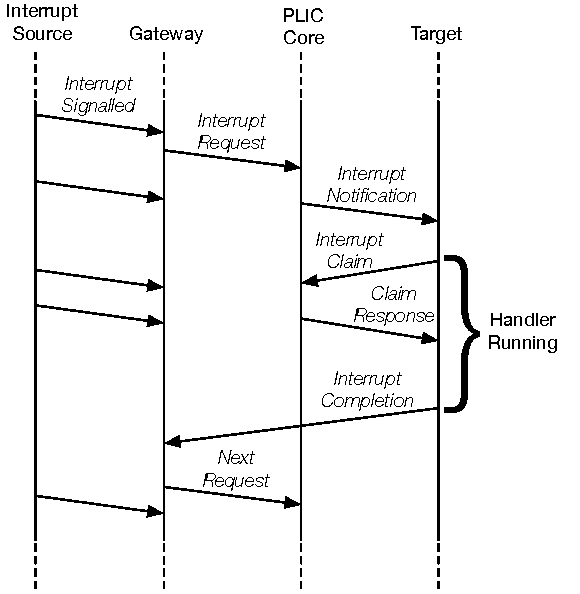
\includegraphics[width=4.0in]{figs/PLIC-interrupt-flow.pdf}
\caption{ Flow of interrupt processing via the PLIC.}
\label{fig:intflow}
\end{figure}

The gateway will only forward a single interrupt request at a time to
the PLIC, and not forward subsequent interrupts requests until an
interrupt completion is received.  The PLIC will set the IP bit once
it accepts an interrupt request from the gateway, and sometime later
forward an interrupt notification to the target.  The target might
take a while to respond to a new interrupt arriving, but will then
send an interrupt claim request to the PLIC core to obtain the
interrupt ID.  The PLIC core will atomically return the ID and clear
the corresponding IP bit, after which no other target can claim the
same interrupt request.  Once the handler has processed the interrupt,
it sends an interrupt completion message to the gateway to allow a new
interrupt request.

\section{PLIC Core Specification}

The operation of the PLIC core can be specified as a non-deterministic
finite-state machine with input and output message queues, with the
following atomic actions:

\begin{itemize}

\item {\bf Write Register: } A message containing a register write
  request is dequeued.  One of the internal registers is written,
  where an internal register can be a priority, an interrupt-enable
  (IE), or a threshold.

\item {\bf Accept Request: } If the IP bit corresponding to the
  interrupt source is clear, a message containing an interrupt request
  from a gateway is dequeued and the IP bit is set.

\item {\bf Process Claim: } An interrupt claim message is dequeued.  A
  claim-response message is enqueued to the requester with the ID of
  the highest-priority active interrupt for that target, and the IP
  bit corresponding to this interrupt source is cleared.

\end{itemize}

The value in the EIP bit is determined as a combinational function of
the PLIC Core state.  Interrupt notifications are sent via an
autonomous process that ensures the EIP value is eventually reflected
at the target. 

Note that the operation of the interrupt gateways is decoupled from
the PLIC core.  A gateway can handle parsing of interrupt signals and
processing interrupt completion messages concurrently with other
operations in the PLIC core.

\begin{commentary}
Figure~\ref{fig:plic} is a high-level conceptual view of the PLIC
design.  The PLIC core can be implemented in many ways provided its
behavior can always be understood as following from some sequential
ordering of these atomic actions.  In particular, the PLIC might
process multiple actions in a single clock cycle, or might process
each action over many clock cycles.
\end{commentary}

\section{Controlling Access to the PLIC}

In the expected use case, only machine mode accesses the source
priority, source pending, and target interrupt enables to configure
the interrupt subsystem.  Lower-privilege modes access these features
via ABI or SBI calls. The interrupt enables act as a protection
mechanism where a target can only signal completion to an interrupt
gateway that is currently enabled for that target.

Interrupt handlers that run with lower than machine-mode privilege
need only be able to perform a claim read and a completion write, and
to set their target threshold value.  The memory map for these
registers should allow machine mode to protect different targets from
each other's accesses, using either physical memory protection or
virtual memory page protections.

